%%%%%%%%%%%%%%%%%%%%%%%%%%%%%%%%%%%%%%%%%%%%%%%%%%%%%%%%%%%
\section{Theory}
\label{sec:theory}
%%%%%%%%%%%%%%%%%%%%%%%%%%%%%%%%%%%%%%%%%%%%%%%%%%%%%%%%%%%

\subsection{Using Boundaries: Friction and Boundary Layers}\label{subsec:WallFriction}
Global inputs move a swarm uniformly.  
Shape control requires breaking this uniform symmetry.  
A swarm inside an axis-aligned rectangular workspace can reduce variance normal to a wall by simply pushing the swarm into the boundary. 
If the swarm can flow around each other, pushing the swarm into a boundary produces the limited set of configurations presented in Sec.~\ref{subsec:FluidInTank}.
%Controlling covariance by pushing the swarm into a boundary requires changes to the boundary.  
%An obstacle in the lower-right corner is enough to generate positive covariance, but generating both positive and negative covariance requires additional obstacles.  
%Requiring a special obstacle configuration also makes shape control dependent on the local environment. 
Instead of pushing our robots directly into a wall, the following sections examine an oblique approach  using boundaries that generate friction with the robots. 
 These frictional forces are  sufficient to break the symmetry caused by uniform inputs.  
Robots touching a wall have a friction force that opposes movement along the boundary.  
This causes robots along the boundary to move more slowly than robots in free-space. 
  
Let the control input be a vector force $\vec{F}$ with magnitude $F$ and orientation $\theta$ with respect to a line perpendicular to and into the nearest boundary. $N$ is the normal or perpendicular force between the robot and the boundary. The force of friction $F_f$ is nonzero if the robot is in contact with the boundary and  $\sin(\theta) < 0$. The resulting net force on the robot, $F_{\text{\emph{forward}}}$, is aligned with the wall and given by
\begin{align}
F_{\text{\emph{forward}}} &=  F \sin(\theta) - F_f  \nonumber \\
\text{where }  F_f &= \begin{cases}  \mu_f N, &  \mu_f N < F \sin(\theta)  \label{eq:frictionmodel}  \\
F \sin(\theta), & \text{else} \end{cases} \\ %\sign(F \sin(\theta) ) \cdot  \max(0, | F sin\theta |- |F_f|)
\text{and } N &= F \cos(\theta) \nonumber
\end{align}
 Fig.~\ref{fig:friction} shows the resultant forces on two robots when one is touching a wall. 
Though each receives the same inputs,  they experience different net forces.
  For ease of analysis, the following algorithms assume $\mu_f$ is infinite and robots touching the wall are prevented from sliding along the wall.
This means that if one robot is touching the wall and another robot is free, the touching robot will not move when the control input is parallel or into the wall. 
There are many alternate models of friction that also break control symmetry. Fig.~\ref{fig:friction}c shows fluid flow along a boundary.  Fluid in the free-flow region moves uniformly, but flow decreases to zero in the boundary layer \citep{fluidMechanics}.  
\begin{align}
%u(y) = u_0 \left(1- \frac{(y-h)^2}{h^2}\right) = u_0 \frac{y}{h} \left(2- \frac{y}{h}\right) \label{eq:boundarylayerflow} THiS EQUATION IS TERRIBLE! PLOT IT.
F_{forward}(y) &= F - F_f\begin{cases}  \frac{h-y}{h}   , &  y<h \label{eq:boundarylayerflow} \\
0, & \text{else} \end{cases}
\end{align}

The next section shows how a system in a rectangularly bounded workspace with friction model \eqref{eq:frictionmodel} can arbitrarily position two robots. 
\begin{figure}[h]
\begin{center}
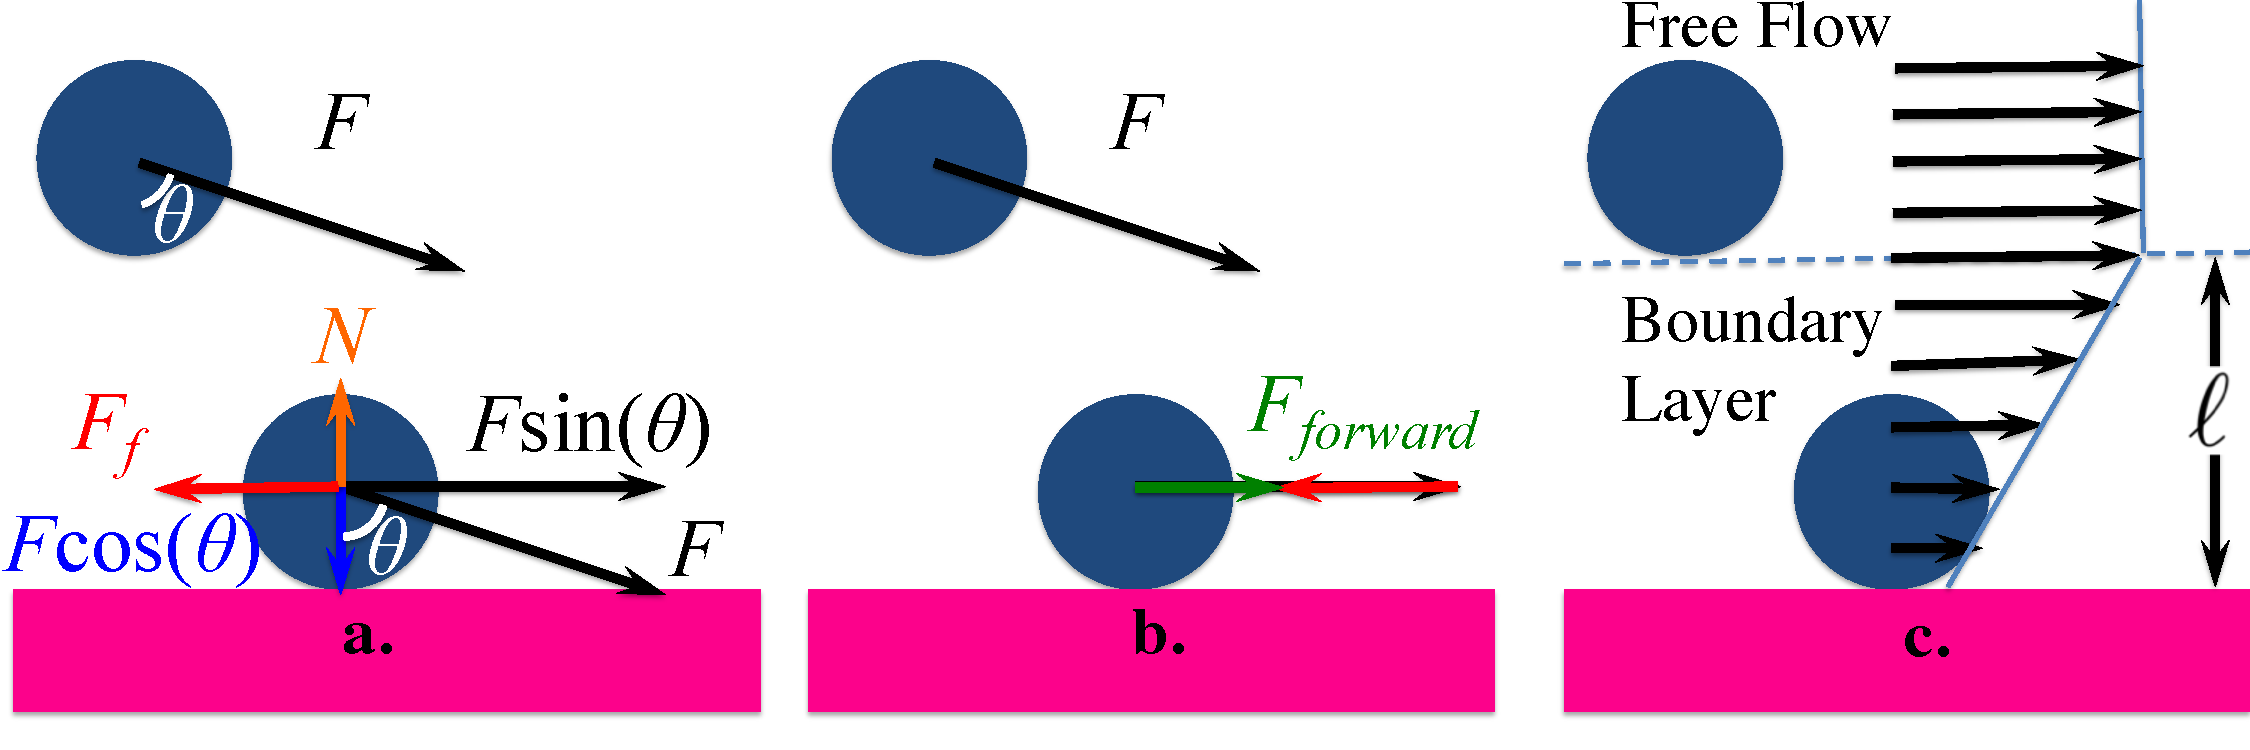
\includegraphics[width=0.8\columnwidth]{friction.pdf} 
\vspace{-1em}
\caption{(a,b) Wall friction reduces the force for going forward $F_{\text{\emph{forward}}}$ on a robot near a wall, but not for a free robot. (c) velocity of a fluid reduces to zero at the boundary.
\label{fig:friction}
}\vspace{-1em}
\end{center}
\end{figure} 



\section{Algorithms}\label{sec:algorithms}
\subsection{Position Control of Two Robots Using Wall Friction}\label{sec:PostionControl2Robots}
\begin{figure*}
\centering
\renewcommand{\figwid}{0.32\columnwidth}
{\begin{overpic}[width =\figwid]{S1.pdf}\put(65,80){Start}
\end{overpic}
\begin{overpic}[width =\figwid]{S2.pdf}\put(50,80){Move 1}
\end{overpic}
\begin{overpic}[width =\figwid]{S3.pdf}\put(50,80){Move 2}
\end{overpic}
\begin{overpic}[width =\figwid]{S4.pdf}\put(50,80){Move 3}
\end{overpic}
\begin{overpic}[width =\figwid]{S5.pdf}\put(50,80){Move 4}
\end{overpic}
\begin{overpic}[width =\figwid]{S6.pdf}\put(50,80){Move 5}
\end{overpic}}\\

\caption{\label{fig:shapeControlMathematica1}{Frames from an implementation of Alg.\ \ref{alg:PosControl2Robots}: two robot positioning using walls with infinite friction. The algorithm only requires friction along the bottom and right walls.
Robot initial positions are shown by a square, and final positions by a circle.  Dashed lines show the shortest route if robots could be controlled independently.  Solid arrows show path given by  Alg.\ \ref{alg:PosControl2Robots}.
Online demonstration and source code at \citep{Shahrokhi2015mathematicaParticle}.
%The bottom row shows an extreme case where the robots must switch position.
}
\vspace{-1em}
}
\end{figure*}

Alg.~\ref{alg:PosControl2Robots} uses wall-friction to arbitrarily position two robots in a rectangular workspace.  This algorithm  introduces concepts that will be used for multi-robot positioning. Fig.~\ref{fig:shapeControlMathematica1} shows a Mathematica implementation of the algorithm, and is useful as a visual reference for the following description.

Assume two robots are initialized at $s_1$ and $s_2$ with corresponding goal destinations $e_1$ and $e_2$. 
We can exploit symmetry in the solution by labeling the leftmost  (or, if they have the same $x$ coordinate, the topmost) robot $s_1$.  If $s_1$ is not also the topmost robot, we rotate the coordinate frame by 90$^\circ$.
Denote the current positions of the robots  $r_1$ and $r_2$. 
Values $.x$ and $.y$ denote the $x$ and $y$ coordinates, i.e., $s_1.x$ and $s_1.y$ denote the $x$ and $y$ locations of $s_1$. Define the sign function as:
\begin{align}
\sign (x) = \begin{cases}  1, &  x > 0 \\
0, & x=0\\
-1, & x<0 \end{cases} 
\end{align}
The algorithm assigns a global control input at every instance.
The goal is to adjust 
 $\Delta r_x = r_2.x-r_1.x$ from $\Delta s_x = s_2.x-s_1.x$ to $\Delta e_x = e_2.x-e_1.x$ and  adjust 
 $\Delta r_y = r_2.y-r_1.y$ from $\Delta s_y = s_2.y-s_1.y$ to $\Delta e_y = e_2.y-e_1.y$ using a shared global control input. 
 This algorithm exploits the position-dependent friction model \eqref{eq:frictionmodel}.
 %employing the assumption we have made earlier about the walls' friction. 

Our algorithm solves the positioning problem in four steps: 
First, it adjusts $\Delta r_y , \Delta r_x$ as much as possible with the left wall.
Second, $\Delta r_x -\Delta e_x$ is reduced to zero with the bottom wall.
Third, if the robots were not correctly positioned relative to each other, $\Delta r_y -\Delta e_y$ is reduced to zero with the right wall.
%First, $|\Delta r_x - \Delta e_x |$ is reduced to zero while  $\Delta r_y$ is kept constant in Alg.~\ref{alg:XControl}. 
%Second, $|\Delta r_y - \Delta e_y |$ is reduced to zero while  $\Delta r_x$ is kept constant. % in Alg.~\ref{alg:YControl}. 
Lastly, the robots, now correctly positioned relative to each other, are moved to their goal locations.

In the worse case, adjusting both $\Delta r_x$ and $\Delta r_y$ needs all four steps. The worst case path length is $2(\sqrt{2}+1)L$.





\begin{algorithm}
\caption{GenerateDesiredSpacing($s_1,s_2,e_1,e_2,L$)}\label{alg:PosControl2Robots}
\begin{algorithmic}[1]
\scriptsize
\Require knowledge of starting $(s_1,s_2)$ and ending $(e_1,e_2)$ positions of  two robots. 
$(0,0)$ is bottom corner, $s_1$ is leftmost robot, 
 $L$ is length of the walls. Current robot positions are $(r_1,r_2)$.
 Assume $s_1.x < s_2.x$ and $s_1.y \geq s_2.y$. If not, rotate workspace coordinates $90^{\circ}$.
$\epsilon $ is a small, nonzero, user-specified value.
 
\Ensure $(e_1, e_2) , (s_1, s_2)$ all at least $\epsilon$ distance from walls.
\State $\Delta e_y = e_2.y - e_1.y$
\State $\Delta e_x = e_2.x - e_1.x$
\State Move $\left(-r_1.x , -\min \left(r_2.y , r_1.y+ \Delta e_y \right)+\epsilon \right)$ \Comment{Touch left wall}
%Second Move
%(-\min(|-r_2.x+ \Delta e_x|, r_2.x),
\State Move $ (r_2.x, |\sign(\Delta e_y)| \, \min(r_1.y - r_2.y + \Delta e_y-\epsilon,L-r_2.y-\epsilon)+ \epsilon)$
\Statex \Comment{Adjust  $y$}
%Third Move
\State Move $(\max(\epsilon, -\sign(r_2.y - r_1.y)\Delta e_x), -\min(r_1.y , r_2.y))$ 
\Statex \Comment{Touch bottom wall}
%Fourth Move
\State Move $(\sign(r_2.y - r_1.y)\Delta e_x , (|\sign(\Delta e_y)|-1) |r_2.y - r_1.y|)$ \Comment{Adjust $x$}
\If {$\Delta e_y \neq r_2.y - r_1.y$}
%Fifth Move
\If {$\Delta e_x \neq 0$}
\State Move $(\sign(r_2.y- r_1.y)\Delta e_x, |\sign(\Delta e_y)-1| |r_1.y-r_2.y|)$ \Comment{Touch right wall}
\Else
\State Move  $(|\sign(\Delta e_y -r_2.y+ r_1.y)| \epsilon, |\sign(\Delta e_y)-1| |r_1.y-r_2.y|)$ \Comment{Touch right wall}
\EndIf
%Sixth Move
\If {$\Delta e_x < 0$}
\State Move $(L - \max(r_1.x, r_2.x), \epsilon)$
\Else 
\State Move $(L - \max(r_1.x, r_2.x),\Delta e_y -\max(r_1.y, r_2.y)$ 
\Statex \Comment{Adjust $y$}
\EndIf
\EndIf
%Seventh Move
\State Move $(e_2.x - r_2.x, e_2.y - r_2.y)$ \Comment{Go to goal}
\end{algorithmic}
\end{algorithm}






\subsection{Position Control of $n$ Robots Using Wall Friction}\label{sec:PostionControlnRobots}
Alg. \ref{alg:PosControl2Robots}  can be extended to control the position of $n$ robots using wall friction under several constraints. The solution described here is an iterative procedure with $n$ loops. The $k$th loop moves the $k$th robot from a \emph{staging zone} to the desired position in a \emph{build zone}. All robots move according to the global input, but due to wall friction, at the end the $k$th loop, robots 1 through $k$ are in their desired final configuration in the build zone, and robots $k+1$ to $n$ are in the staging zone. See Fig.~\ref{fig:construction2d} for a schematic of the build and staging zones.
\begin{figure}
\begin{center}
	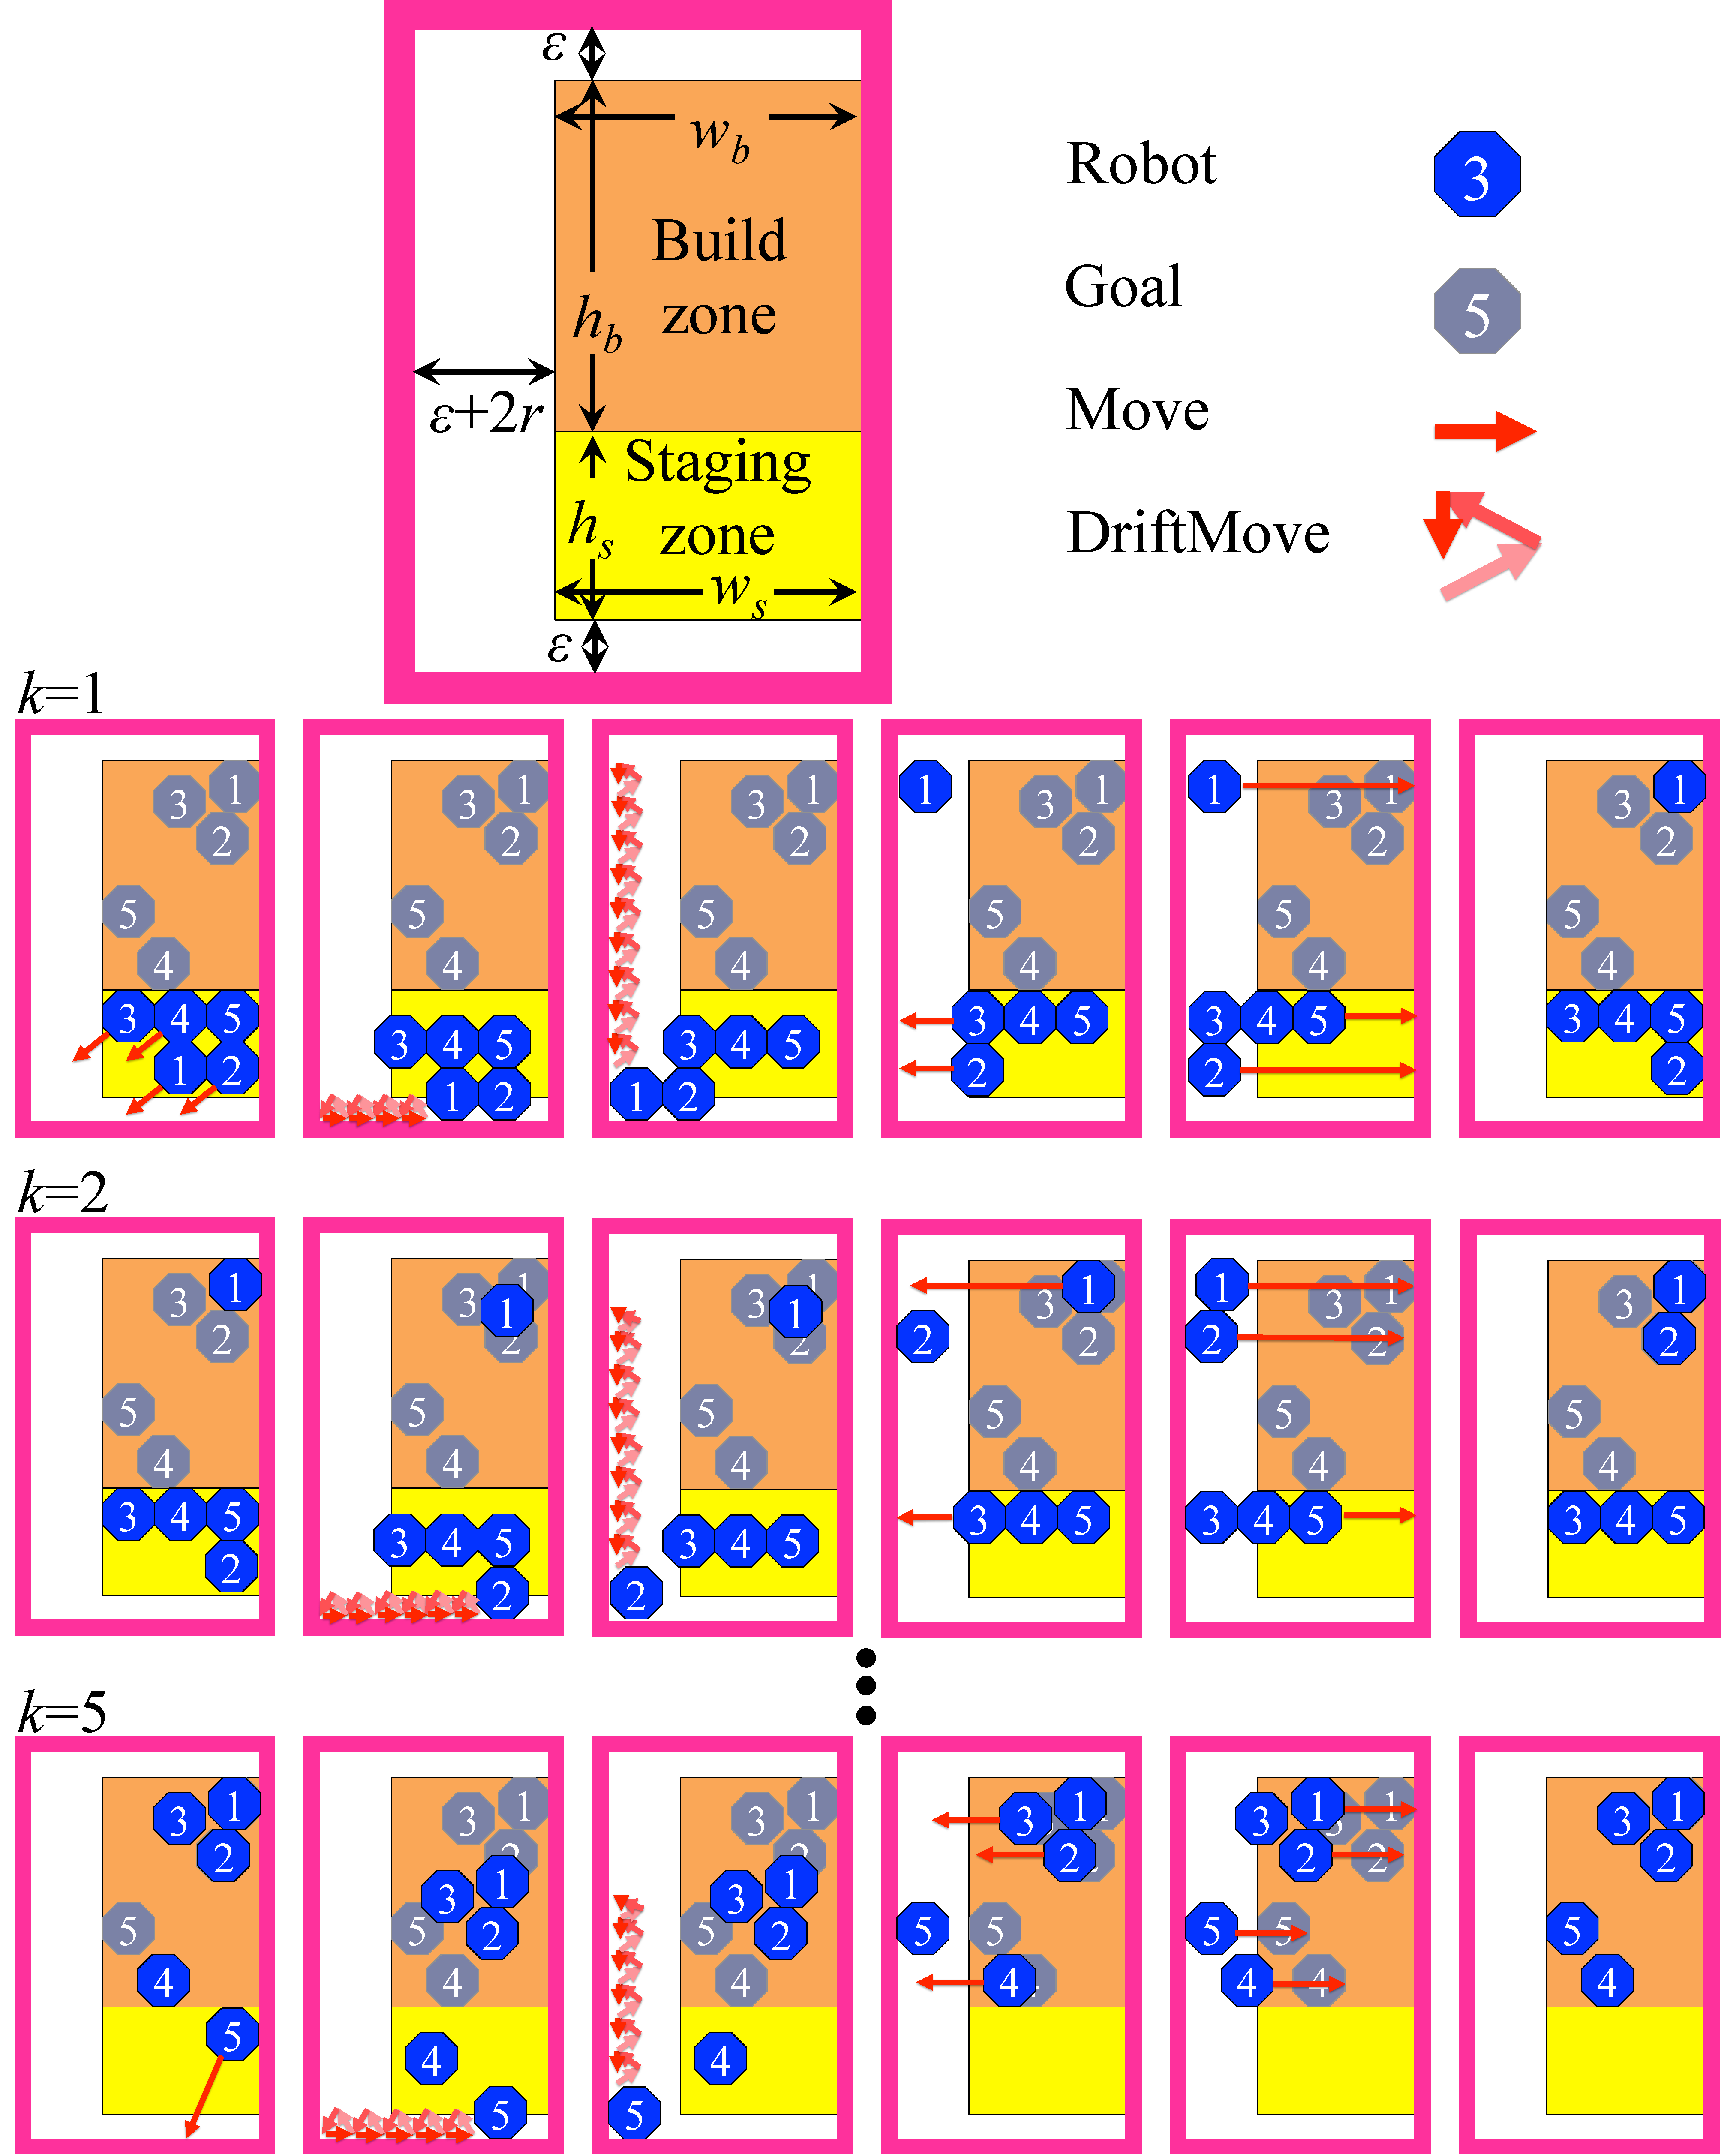
\includegraphics[width=1.0\columnwidth]{PositionNrobotsComp.pdf}
\end{center}
\vspace{-1em}
\caption{\label{fig:simulationNrobot}
Illustration of Alg.\ \ref{alg:PosControlNRobots}, $n$ robot position control  using wall friction.
}
\end{figure}

\begin{figure}
\begin{center}
	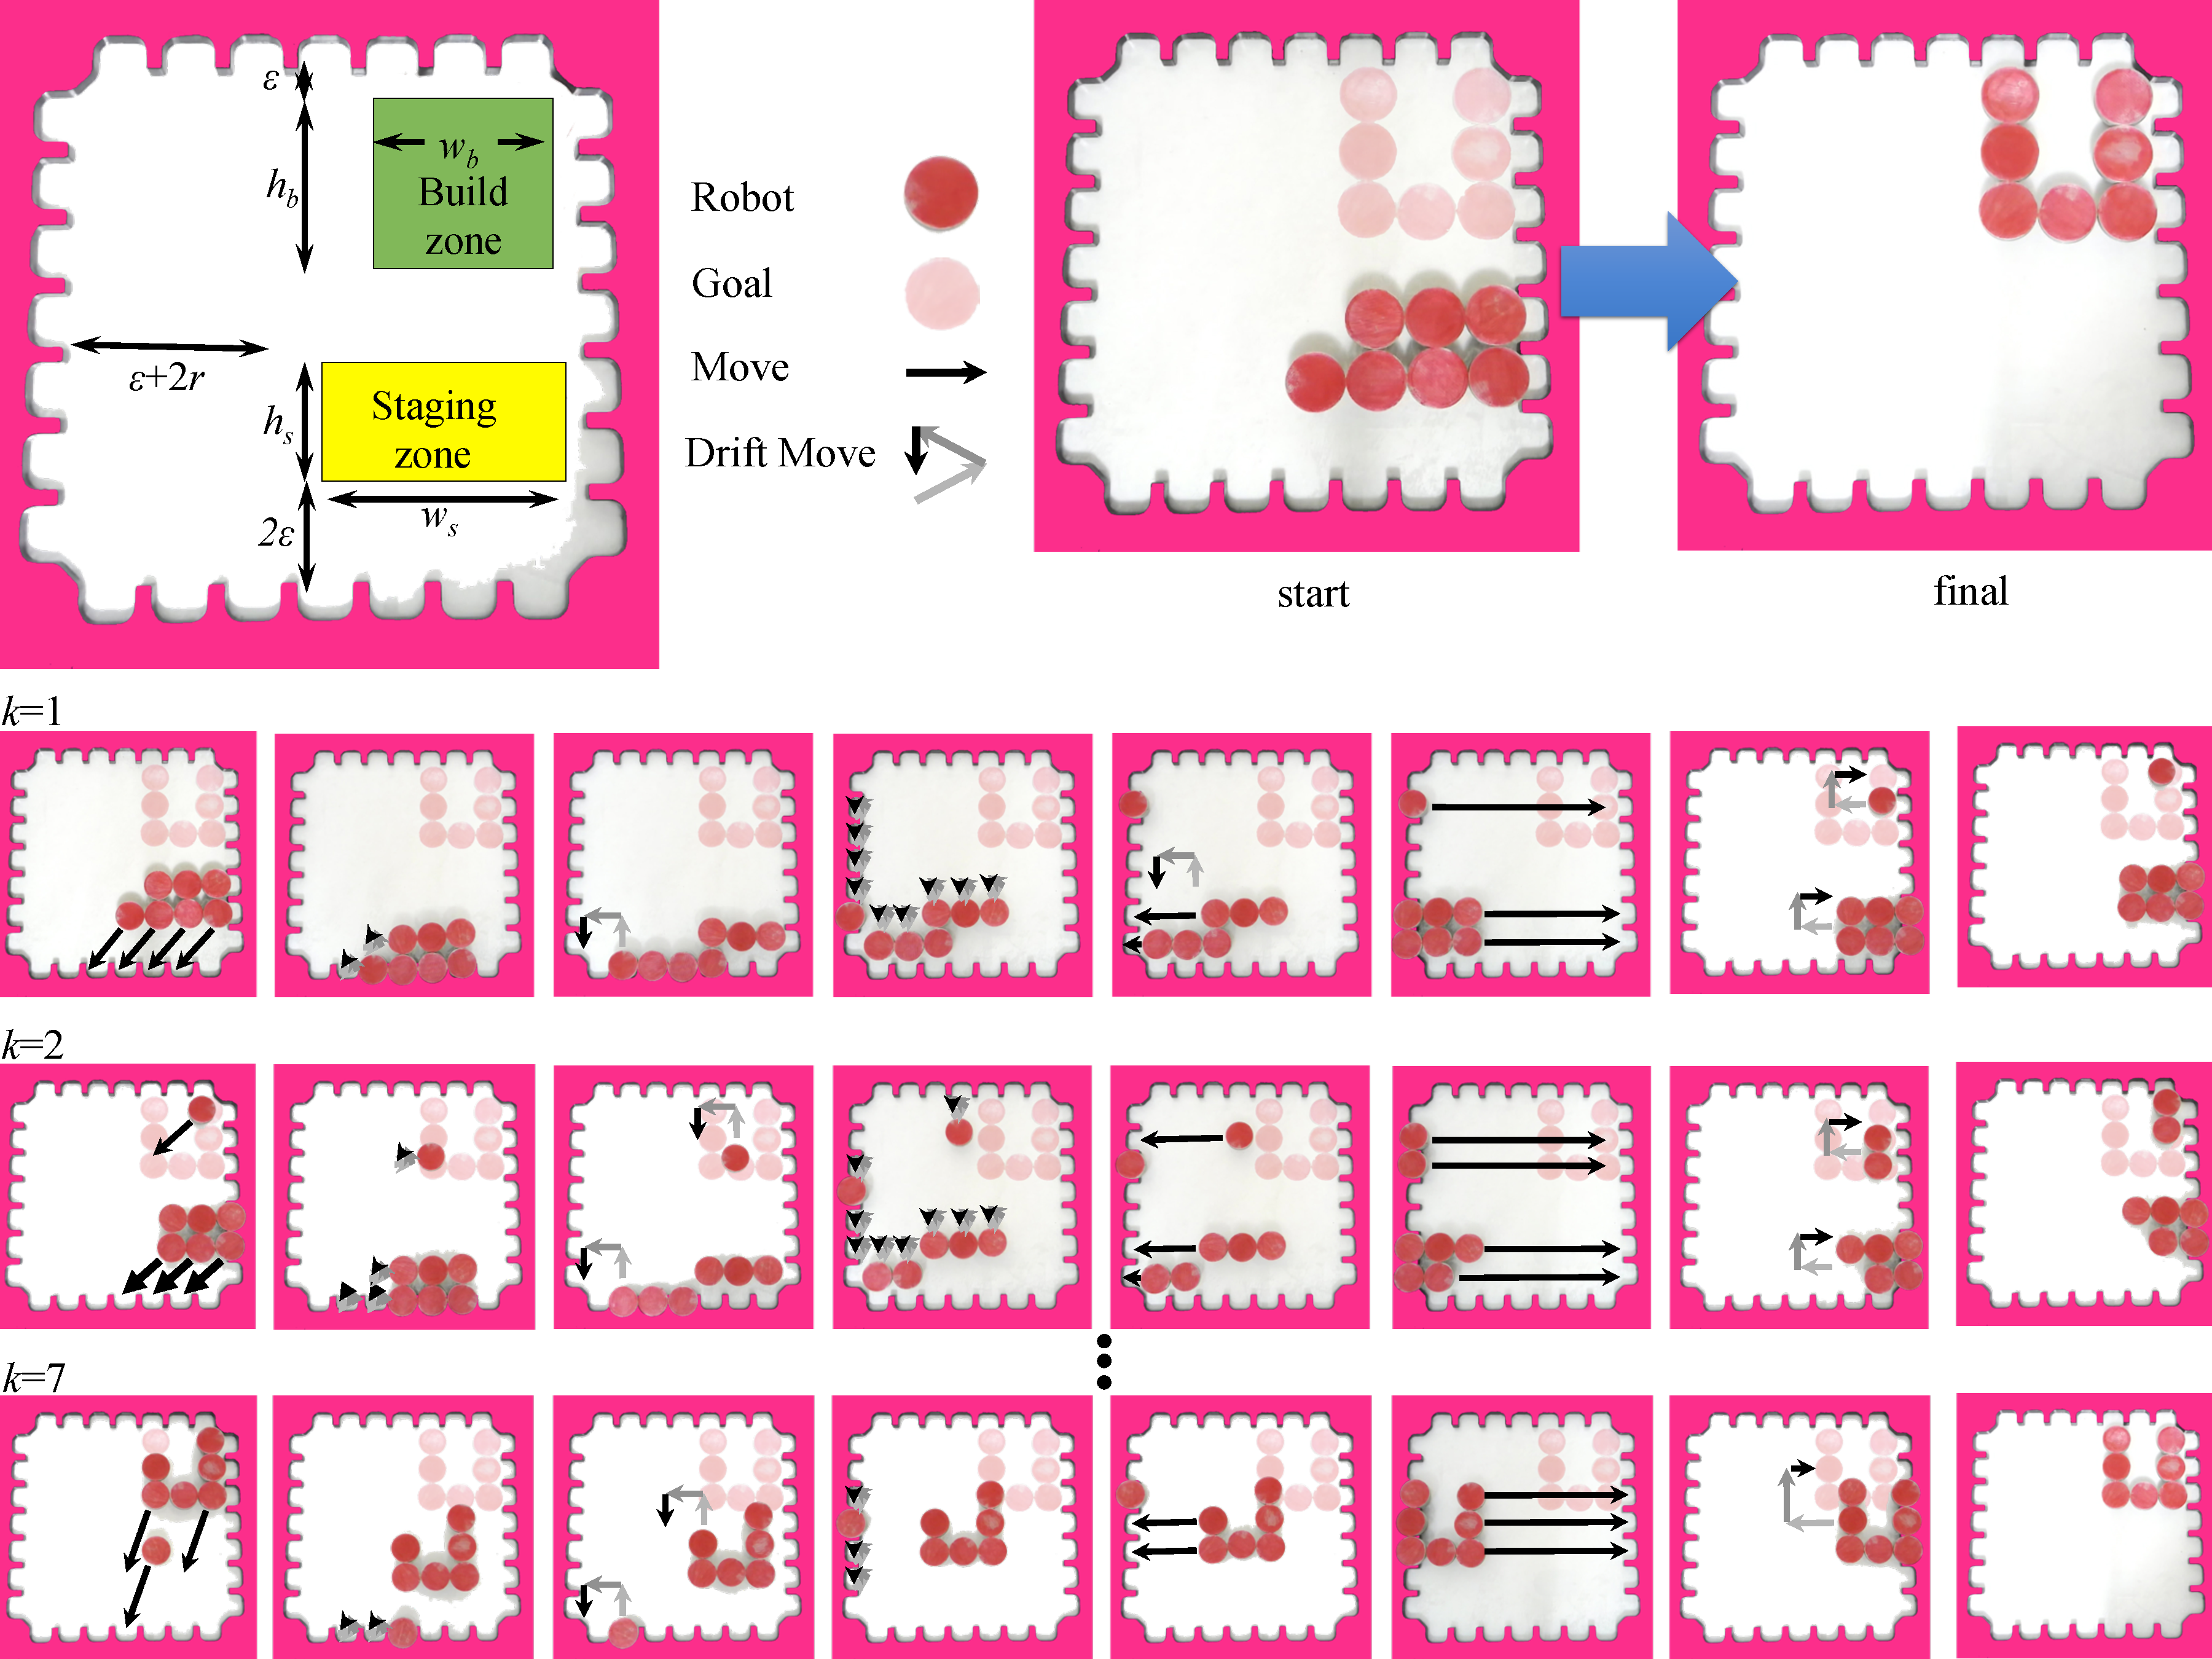
\includegraphics[width=1.0\columnwidth]{multirobotSliderHardware.pdf}
\end{center}
\vspace{-1em}
\caption{\label{fig:construction2d}
Illustration of Alg.\ \ref{alg:PosControlNRobots}, $n$ robot position control  using wall friction.
}
\end{figure}




Assume an open workspace with four axis-aligned walls with infinite friction.
The axis-aligned build zone of dimension $(w_b, h_b)$ containing the final configuration of $n$ robots must be disjoint from the axis-aligned staging zone of dimension $(w_s, h_s)$  containing the starting configuration of $n$ robots. Without loss of generality, assume the build zone  is above the staging zone. 
Furthermore, there must be at least $\epsilon$ space above the build zone, $\epsilon$ below the staging zone, and $\epsilon + 2r$ to the left of the build and staging zone, where $r$ is the radius of a robot.  The minimum workspace is then $(\epsilon + 2r + \max(w_b,w_s), 2\epsilon + h_s,h_b)$.

The $n$ robot position control algorithm relies on a $\operatorname{DriftMove}(\alpha, \beta, \epsilon)$ control input, shown in Fig.\  \ref{fig:driftmove}.
A drift move consists of repeating a triangular movement sequence $\{ (\beta/2,-\epsilon),(\beta/2,\epsilon),(-\alpha,0)\}$. The robot touching a top wall moves right $\beta$ units, while robots not touching the top move right $\beta-\alpha$.

\begin{figure}
\begin{center}
	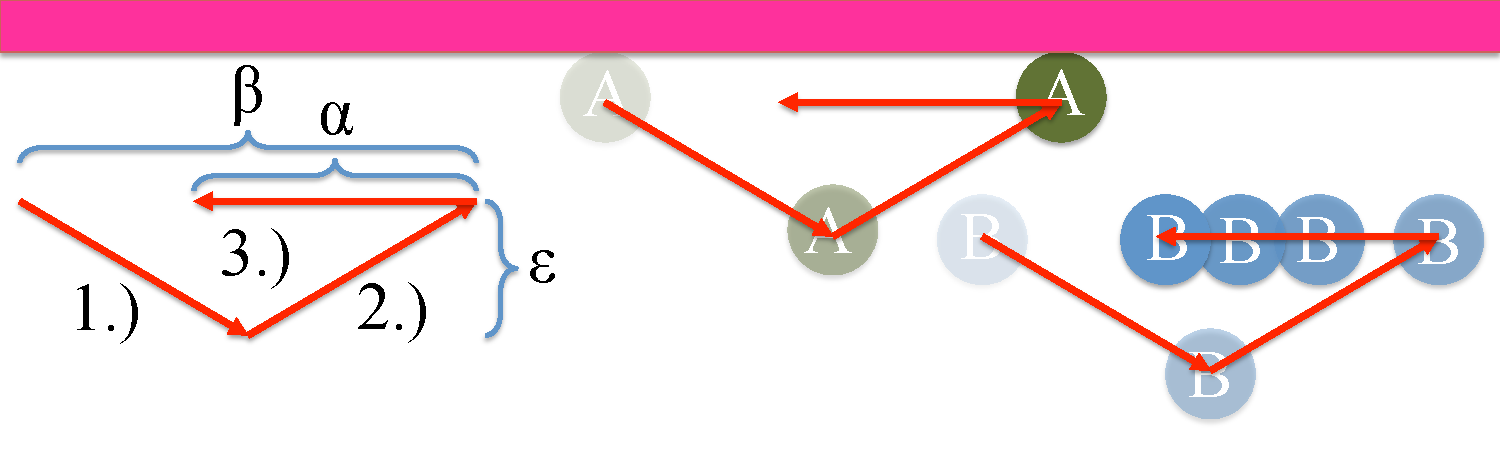
\includegraphics[width=.9\columnwidth]{driftmove.pdf}
\end{center}
\vspace{-1em}
\caption{\label{fig:driftmove}
A  $\operatorname{DriftMove}(\alpha, \beta, \epsilon)$ to the right repeats a triangular movement sequence $\{ (\beta/2,-\epsilon),(\beta/2,\epsilon),(-\alpha,0)\}$. Robot $A$ touching a top wall moves right $\beta$ units, while robots not touching the top move right $\beta-\alpha$.}
\vspace{-1em}
\end{figure}

Let $(0,0)$ be the lower left corner of the workspace, $p_k$ the $x,y$ position of the $k$th robot, and $f_k$ the final $x,y$ position of the $k$th robot. Label the robots in the staging zone from left-to-right and bottom-to-top, and the $f_k$ configurations top-to-bottom and right-to-left as shown in Fig.~\ref{fig:construction2d}.

\begin{algorithm}
\caption{PositionControl$n$RobotsUsingWallFriction($k$)}\label{alg:PosControlNRobots}
\begin{algorithmic}[1]
\State Move( $-\epsilon, r-p_{ky}$) % move  away from right wall and down till robot k touches bottom


\While{ $p_{kx} > r$} 
\State $\operatorname{DriftMove}(\epsilon, \min(p_{kx} - r,\epsilon), \epsilon,left)$    %drift move left until kth robot touches left wall
\EndWhile

\State $m \gets \operatorname{ceil}(\frac{f_{ky}-r}{\epsilon})$
\State $\beta \gets \frac{f_{ky}-r}{m}$
\State $\alpha \gets \beta - \frac{r - p_{ky}-\epsilon}{m}$
\For{ $m$ iterations}
\State $\operatorname{DriftMove}(\alpha, \beta, \epsilon,up)$    %move kth robot to f_{ky} and leave the rest in position.
\EndFor

\State Move ($r+\epsilon-f_{kx}, 0$)  % move the group to the left until k is in the correct relative x position
\State Move ($f_{kx}-r, 0$)  

\end{algorithmic}
\end{algorithm}


\begin{algorithm}
\caption{ {\sc DriftMove}($\alpha,\beta,\epsilon,direction$)}\label{alg:DriftMove}
\begin{algorithmic}[1]
\State Move( $-\epsilon, r-p_{ky}$) % move  away from right wall and down till robot k touches bottom
\State Move ($r+\epsilon-f_{kx}, 0$)  % move the group to the left until k is in the correct relative x position
\State Move ($f_{kx}-r, 0$)  

\end{algorithmic}
\end{algorithm}


Alg. \ref{alg:PosControlNRobots} proceeds as follows:  
First, the robots are moved left away from the right wall, and down so robot $k$ touches the bottom wall.
Second, a set of $\operatorname{DriftMove}$s are executed that move robot $k$ to the left wall with no net movement of the other robots.
Third, a set of $\operatorname{DriftMove}$s are executed that  move robot $k$ to its target height and return the other robots to their initial heights. 
Fourth, all robots except robot $k$ are pushed left until robot $k$ is in the correct relative $x$ position compared to robots 1 to $k-1$.
Finally, all robots are moved right until robot $k$ is in the desired target position. Running time is $O(n(w+h))$.



